\chapter{Plonk Proof System}
This section provides an overview of the PLONK proof system for arithmetic circuits.
In this chapter, we assume the existence of a polynomial commitment scheme (e.g., the KZG commitment scheme) and show how to use such a commitment to construct the PLONK proof system.

Throughout this chapter, we denote the commitment of polynomial function $f$ as $com_f$.

\section{Vanishing Polynomial}
Let $\F_p$ be a field of large prime order $p$, and let $\Omega \subseteq \F_p$ be a subset with $|\Omega| = k$.
In the following sections, we define efficient polynomial IOPs (Interactive Oracle Proofs) for various tasks over $\Omega$. 

\begin{remark}
    Using a specific subset $\Omega$ rather than the entire field $\F_p$ allows us to work with a manageable set of evaluation points. 
    If the entire field were used, the corresponding vanishing polynomial would have degree $p$, which is impractical for computation.
\end{remark}

\begin{definition} [Vanishing Polynomial]
    The \textit{vanishing polynomial} of $\Omega$, denoted by $Z_{\Omega}(X)$, is the unique polynomial that evaluates to zero at every point in $\Omega$. 
Thus, we have
\[
    Z_{\Omega}(X) = \prod_{a \in \Omega} (X - a),
\]
which implies that the degree of $Z_{\Omega}(X)$ is $|\Omega|$.
\end{definition}


For the specific case where $w$ is a primitive $k$th root of unity (i.e., $w^k = 1$) and 
\[
    \Omega = \{1, w, w^2, \ldots, w^{k-1}\} \subset \F_p,
\]
the vanishing polynomial simplifies to
\[
    Z_{\Omega}(X) = X^k - 1.
\]

\begin{remark}
    In the case where $\Omega = \{1, w, w^2, \ldots, w^{k-1}\}$, the vanishing polynomial can be evaluated efficiently using exponentiation by squaring, which requires approximately $\log_2 k$ multiplications; when counting both squaring and multiplication steps, the total comes to roughly $2\log k$ operations. 
    In contrast, for a general subset $\Omega$, directly computing 
    \[
    Z_{\Omega}(X) = \prod_{a \in \Omega} (X - a)
    \]
    would require $k-1$ multiplications, making it much less efficient for large $k$.
\end{remark}

This significant speedup is why, in the subsequent sections, we restrict ourselves to the case
\[
    \Omega = \{1, w, w^2, \ldots, w^{k-1}\}.
\]


\section{Zero Test}
Assume a prover \(P\) wants to prove to a verifier \(V\) that 
\[
    f(a) = 0 \quad \text{for all} \; a \in \Omega,
\]
and the verifier already holds a commitment \(\text{com}_f\) to the polynomial \(f\).
Let \(\Omega \subset \F_p\) be a subset of size \(\lvert \Omega \rvert = k\), and assume \(\deg(f) \le d\).

The naive approaches for the verifier are:
\begin{enumerate}
    \item The verifier directly evaluates \(f\) on every point in \(\Omega\) and checks if each evaluation is zero. 
    This requires \(\mathcal{O}(k)\) polynomial evaluations, which is inefficient for large \(k\).
    \item The verifier queries the prover to prove correctness of \(f(a)=0\) for each \(a \in \Omega\). 
    This yields \(\mathcal{O}(k)\) individual proofs, also inefficient.
\end{enumerate}

By using an Interactive Oracle Proof (IOP) and a vanishing polynomial, we can reduce the complexity significantly. 
The key observation is:
\[
    \text{If } f(a) = 0 \; \text{for all} \; a \in \Omega, 
    \quad \text{then} \quad 
    f(X) = q(X)\,\cdot Z_{\Omega}(X),
\]
where \(Z_{\Omega}(X)\) is the vanishing polynomial over \(\Omega\). 


\begin{center}
    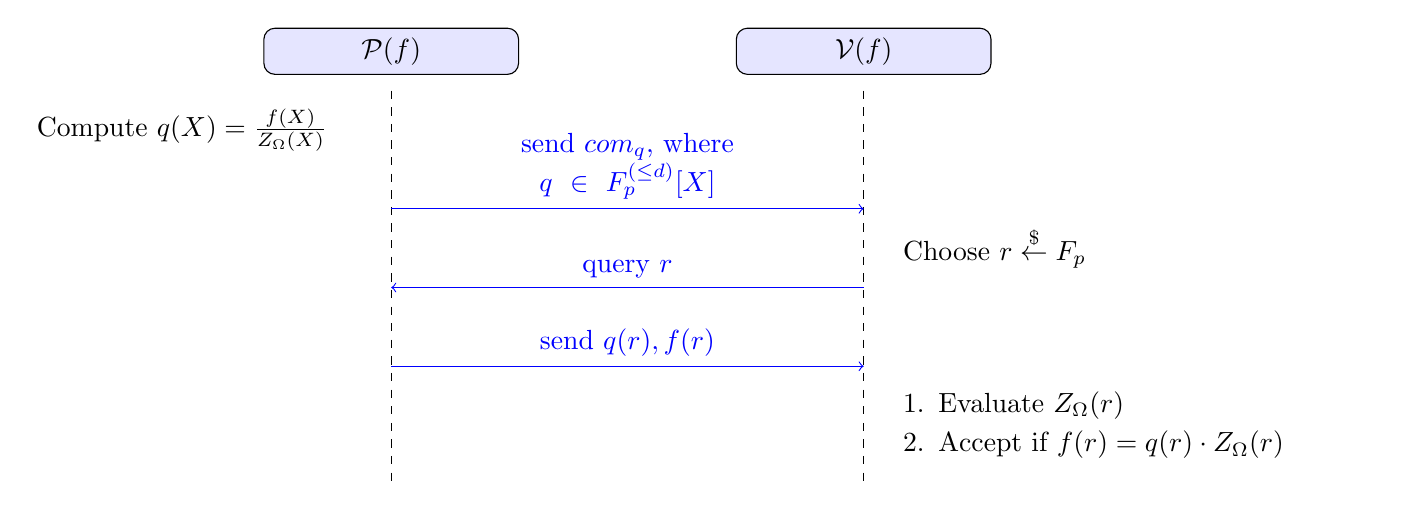
\begin{tikzpicture}[node distance=1.5cm, xshift=-3cm]
    
    % Define styles
    \tikzstyle{actor} = [rectangle, draw, rounded corners, fill=blue!10, minimum height=1em, text width=3cm, align=center]
    \tikzstyle{action} = [text width=6cm, align=left]
    
    % Prover and Verifier headers with lifelines
    \node[actor] (prover) at (0,0) {$\mathcal{P}(f)$};
    \draw[dashed] (0,-0.5) -- (0,-5.5);
    
    \node[actor] (verifier) at (6,0) {$\mathcal{V}(f)$};
    \draw[dashed] (6,-0.5) -- (6,-5.5);
    
    % Prover computes q(X)
    \node[action] at (-1.5,-1) {Compute $q(X) = \frac{f(X)}{Z_\Omega(X)}$};
    
    % Prover sends q to Verifier
    \draw[->, blue] (0,-2) -- node[midway, above, text width=4cm, align=center] {send $com_q$, where $q \in \mathbb{F}_p^{(\leq d)} [X]$} (6,-2);
    
    % Verifier chooses r
    \node[action] at (9.5,-2.5) {Choose $r \stackrel{\$}{\leftarrow} \mathbb{F}_p$};
    
    % Verifier queries r to Prover
    \draw[->, blue] (6,-3) -- node[midway, above] {query $r$} (0,-3);
    
    % Prover responds with q(r), f(r)
    \draw[->, blue] (0,-4) -- node[midway, above] {send $q(r), f(r)$} (6,-4);
    
    % Verifier evaluates Z_\Omega(r)
    \node[action] at (9.5,-4.5) {1. Evaluate $Z_\Omega(r)$};
    
    % Verifier checks acceptance condition
    \node[action] at (9.5,-5) {2. Accept if $f(r) = q(r) \cdot Z_\Omega(r)$};
    
    \end{tikzpicture}
\end{center}

\subsubsection*{Protocol Overview}
\begin{enumerate}
    \item \textbf{Compute and Commit to \(q\):} 
        The prover computes the polynomial \(q(X)\) such that \(f(X) = q(X)\,Z_{\Omega}(X)\). 
        Since \(\deg(f) \le d\), we have \(\deg(q) \le d\). 
        The prover sends a \emph{commitment} to \(q\) (denoted \(\text{com}_q\)) to the verifier.
    \item \textbf{Random Challenge:} 
        The verifier samples a random challenge \(r \in \F_p\) (public-coin protocol). 
        The verifier sends \(r\) to the prover.
    \item \textbf{Opening the Commitments:}
        The prover returns:
        \[
            f(r), \quad q(r),
        \]
        along with proofs (in the polynomial commitment scheme) that these openings are consistent with the committed polynomials \(f\) and \(q\). 
        This ensures the prover cannot lie about the polynomial values.
    \item \textbf{Check the Factorization:}
        The verifier locally computes \(Z_{\Omega}(r)\). 
        Then it checks the relation
        \[
            f(r) \stackrel{?}{=} q(r)\cdot Z_{\Omega}(r).
        \]
        If this holds, the verifier accepts; otherwise, it rejects.
\end{enumerate}

\begin{proof}[Informal Security Argument]
    If \(f(X)\) truly vanishes on \(\Omega\), then there is a valid \(q(X)\) of degree at most \(d\), and the relation \(f(r) = q(r)\,Z_{\Omega}(r)\) holds for all \(r\). The verifier accepts.
 
    Conversely, define
    \[
        h(X) \;=\; f(X)\;-\;q(X)\,Z_{\Omega}(X).
    \]
    If \(f(X)\) does \emph{not} vanish on \(\Omega\), then no polynomial \(q(X)\) of degree at most \(d\) can satisfy \(f(X) = q(X)\,Z_{\Omega}(X)\). 
    Consequently, \(h(X)\) is a nonzero polynomial. 
    A nonzero polynomial of degree \(\deg(h)\) over \(\F_p\) can have at most \(\deg(h)\) roots. 
    Hence, when the verifier selects a random \(r\in \F_p\), the probability that \(h(r) = 0\) is at most \(\deg(h)/|\F_p|\). 
    Therefore, except with negligible probability, the verifier's check 
    \[
        f(r) \stackrel{?}{=} q(r)\,Z_{\Omega}(r)
    \]
    will fail, and the verifier will reject.
\end{proof}

\section{Product Check}

\section{Premutation Check}

\section{Prescribed Permutation Check}